\chapter{Introdução}
\label{cap:introducao}

Os sistemas de transporte estabeleceram-se ao longo dos anos como um dos principais condicionantes ao desenvolvimento socioeconômico mundial. Em sua utilização, seja para circulação de pessoas ou escoamento de produção, intensifica-se cada vez mais demandas por eficiência, dado seu fator estratégico. Neste contexto, com a agregação de tecnologias computacionais surgiram os Sistemas de Transporte Inteligentes (STI), onde através de sensoriamento em veículos e na infraestrutura de transporte são produzidas informações em tempo-real para tomada de decisão. Estas informações são utilizadas tanto por usuários do modal, quanto operadores e administradores do sistema de transporte \cite{NI2016}.

As informações produzidas consistem de dados situacionais sobre o ambiente de trânsito e de seus participantes. Estas informações possuem grande aplicabilidade, com impactos sociais, econômicos e ambientais. No suporte à tomada de decisão humana, dados como qualidade do pavimento e geolocalização de obstáculos e irregularidades na pista podem ser empregados para planejamento de rotas no escoamento de produção, uma vez que o inadequado estado de conservação do pavimento produz, em média, elevação de 27,0\% dos custos operacionais \cite{CNT2017}. Estes dados também podem ser utilizados por administradoras da via para planejamento de manutenções ou por usuários em sistemas de assistência à condução, melhorando a segurança no trânsito. No suporte à tomada de decisão de máquina, além dos dados supracitados, outros como tipo de pavimento e perfil de condução podem ser utilizados em veículos autônomos para coordenar suas ações.

Para produção dos dados brutos que, após processados, geram as informações do STI, diversas tecnologias foram propostas. Dentre as classificações existentes, pode-se categorizá-las entre abordagens intrusivas e não intrusivas \cite{NI2016}, conforme ilustra a Figura \ref{fig:classificacao_sensores}. Na abordagem intrusiva, os dados brutos são amostrados de sensores colocados diretamente na superfície de via, requerendo possíveis alterações no pavimento ou no tráfego \cite{mathew2014a}. Já na abordagem não-intrusiva, não são realizadas alterações na infraestrutura da via, com os sensores colocados dentro dos veículos que nela trafegam \cite{mathew2014b}. Os métodos não intrusivos possuem diversas vantagens em relação aos intrusivos, tais como serem menos onerosos, de fácil instalação, cobrirem uma área de monitoramento muito maior e permitirem, além da inspeção da infraestrutura, o acompanhamento das ações dos participantes através da propriocepção.

Na abordagem não intrusiva, são empregadas técnicas com estratégias passivas ou ativas. As técnicas ativas requerem interação com o ambiente para produzir seus dados brutos, como emissão de ondas na superfície de pista através de laser ou radar. As técnicas passivas, por sua vez, não requerem interação com o ambiente, amostrando dados físicos ou de imagens. Em contraste com as técnicas ativas, as passivas são consideradas não poluentes, sendo ideais para uso em larga escala. Desta forma, para uma maior aplicação do STI, tais como veículos autônomos, é necessário que se desenvolva cada vez mais tecnologias menos poluentes. Entretanto, embora a visão computacional tenha nos últimos anos progredido bastante sobre os dados de imagens, dados físicos obtidos através de sensores inerciais tem sido pouco explorados, limitando-se a estudos exploratórios de aplicabilidade.

\begin{figure}[t]
  \centering
  \caption{Abordagens de sensoriamento em STI.}
  \label{fig:classificacao_sensores}
  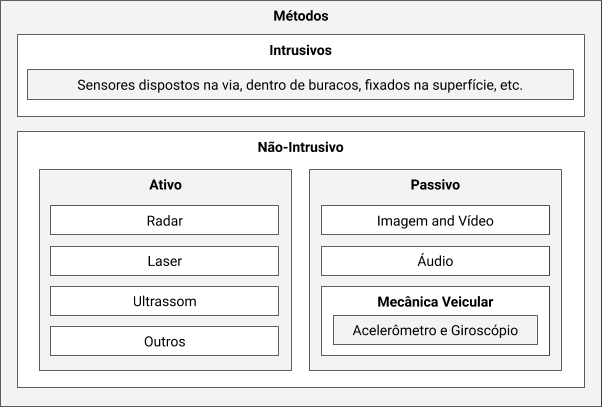
\includegraphics[width=0.9\linewidth]{figuras/fig1.png}
  \fonte{O autor.}
\end{figure}

\section{Contextualização do Problema}

Classificados como não-intrusivos e passivos, os sensores inerciais se baseiam no princípio da inércia para produção de seus dados \cite{Braga2017}. Sendo assim, representados por acelerômetros e giroscópios, estes dispositivos produzem sinais unidimensionais referentes a taxa de rotação e a força de aceleração respectivamente, em seus três eixos físicos \cite{Groves2013}. Dentre suas diversas aplicações em STI, as principais estão internamente aos automóveis, seja fixados diretamente na estrutura veicular ou embarcados em dispositivos móveis, como \textit{smartphones} e \textit{tablets}.

Os dados obtidos através destes sensores, após processados, geram informações que podem ser classificadas entre percepção de ambiente e propriocepção, conforme detalha a Figura 2. As percepções de ambiente buscam compreender o ambiente fora do veículo, realizando o reconhecimento de características do caminho no qual trafega. Estas características incluem eventos transientes, como anomalias e obstáculos; e persistentes, como tipo de composição e qualidade de superfície de pista. A propriocepção, por sua vez, objetiva compreender os movimentos veiculares para identificar seu próprio comportamento. Estas identificações também podem ser transientes, como eventos de condução; e persistentes, como perfil de comportamento de condução.

\begin{figure}[t]
  \centering
  \caption{Percepções veiculares através de sensoriamento inercial.}
  \label{fig:percepcoes_veiculares}
  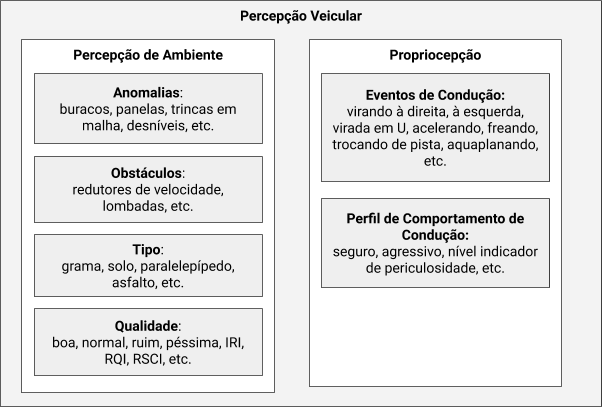
\includegraphics[width=0.9\linewidth]{figuras/fig1_1.png}
  \fonte{O autor.}
\end{figure}

Embora sejam diversas e relevantes as percepções veiculares produzidas, a utilização de sensores inerciais em STI pouco avançou nos últimos anos. A maioria dos estudos da área obtidos através da Revisão Sistemática da Literatura (RSL) possuí foco na aplicabilidade das percepções produzidas, consistindo de estudos com viés exploratório, não havendo um modelo realmente confiável para aplicação real. Sendo assim, são diversas as lacunas de pesquisa existentes, sendo a principal delas a necessidade da produção de um modelo adaptativo com alto grau de confiabilidade quando aplicado em cenários não controlados.

Para que se possa disseminar a aplicação de sensores inerciais em STI, ampliando a utilização de sensoriamento não poluente, a adaptabilidade é um fator essencial. Sendo assim, é necessário se desenvolver um modelo que permita um alto nível de adaptabilidade, considerando seus fatores de dependência, situado em um contexto extremamente dinâmico. Estes fatores são considerados propriedades sensoriais como faixas de medição, resolução, referenciais de captação e análise; propriedades ambientais, como alterações de tipo de pavimentação e condições climáticas; propriedades veiculares, como sistema de suspensão e mecânica veicular; além das propriedades de condução, como velocidade aplicada ao veículo.

\section{Objetivos}

Nesta seção são detalhados o objetivo geral e específicos desta pesquisa.

\subsection{Objetivo Geral}

Este trabalho objetiva desenvolver um modelo adaptativo de percepção de ambiente e propriocepção veicular baseado em sensoriamento inercial e Inteligência Artificial, de forma a realizar percepções com alto grau de confiabilidade, independente do contexto ou outras fontes de dados.

\subsection{Objetivos Específicos}

Os objetivos específicos deste trabalho são:

\begin{itemize}

\item Identificar o estado da arte na produção de percepção veicular através da utilização de sinais de sensores inerciais, nas etapas de coleta, pré-processamento e processamento;

\item Desenvolver uma metodologia para captação de dados, compreendendo a criação e configuração de uma rede com sensores inerciais e de localização, sua distribuição e posicionamento na estrutura veicular.

\item Produzir nove conjuntos de dados com variações ambientais, de condução e de veículos.

\item Desenvolver etapa de pré-processamento, objetivando melhorar os dados brutos dos sensores, assim como sua segmentação, georreferenciamento e normalização;

\item Investigar combinação de técnicas de reconhecimento de padrões para realizar percepção veicular de ambiente e propriocepção, treinando e validando através dos conjuntos de dados produzidos;

\item Investigar a integração entre percepções transientes e persistentes, assim como integração de percepção de ambiente com propriocepção, afim de melhorar a confiabilidade do modelo;

\item Propor um modelo adaptativo de percepção veicular ampla e integrada, situando os melhores modelos dado os pontos de captação e tipo de aplicação;

\end{itemize}

\section{Justificativa}

Para desenvolvimento dos STI e sua ampla disseminação, se faz necessário ter cada vez mais fontes de dados, que estes dados sejam confiáveis, e que os dispositivos que os produzem não sejam prejudiciais à saúde humana. Sendo assim, constituindo um meio de baixo custo e não poluente, o emprego dos sensores inerciais na geração de percepção veicular para os STIs se mostra de grande contribuição, seja para tomada de decisão humana ou de máquina.

Com o desenvolvimento de um modelo adaptativo de percepção, constituindo um aplicação meio para outros sistemas, diversas áreas dos STIs podem se beneficiar, como Sistemas Avançados de Gerenciamento de Tráfego (SAGT), Sistemas Avançados de Assistência ao Motorista (SAAM), sistemas de transporte público, sistema de gestão de infraestrutura, veículos autônomos, caixas preta veiculares, sistemas de gestão de escoamento de produção, entre diversos outros.

\subsection{Cenários de Aplicação}

Nesta seção são detalhados alguns cenários de aplicação do modelo proposto.

\begin{description}

\item [Navegação Autônoma:] Um veículo equipado com sensores inerciais e auxiliares de suporte trafega em uma via. A irregularidade longitudinal da pista, correspondente ao conjunto dos desvios da superfície, é processada em relação à um plano de referência. Nesta análise, é estabelecido um índice de qualidade de conservação e identificado o tipo de pavimentação da via. Também são reconhecidos e classificados eventos transientes de percepção de ambiente, como obstáculos na via (lombadas, redutores de velocidade, etc.), deficiências da superfície (buracos, solavancos, etc.); e de propriocepção, como eventos de condução (virando à direita suave ou bruscamente, virando à esquerda, acelerando, frenando, etc). Disponibilizando estas informações através de uma interface ao agente inteligente que controla o veículo, o índice de qualidade de superfície e o tipo de pavimentação aferido são empregados no controle de velocidade veicular, sendo menor em vias mais irregulares e vice-versa. Esta decisão pode ser monitorada através dos eventos de condução e, se necessário, efetuado ajustes de comando. Os eventos transientes detectados de percepção de ambiente, utilizados na forma de evidências, auxiliam na convalidação de dados obtidos de sensores multimodais, tal qual por intermédio de visão computacional, corroborando hipóteses sobre o contexto no qual está inserido.

\item [Sistema Avançado de Assistência ao Motorista:] Em um sistema de \textit{vehicular crowdsensing} com sensoriamento oportunista, um \textit{crowdsourcer} utiliza um aplicativo de Sistema Avançado de Assistência ao Motorista (\textit{Advanced Driver Assist System} - ADAS) em seu computador de bordo. Com os sensores inerciais anexados ao veículo, o aplicativo analisa as vibrações recebidas, para estabelecer conceitos qualitativos sobre a irregularidade de superfície e reconhecer eventos transientes, na forma de obstáculos e anomalias. Um servidor central recebe dados de vários \textit{crowdsourcers}, onde aplica-se um aprendizado baseado em reforço. Empregando a confiabilidade inicialmente estalecida e a quantidade de detecções em diferentes fontes, a aplicação central realiza ajustes periódicos dos valores de confiabilidade dos dados, de forma que falsos positivos tenham progressivamente sua confiabilidade reduzida a zero, assim como algum evento transientes que deixe de existir, especialmente em função das manutenções realizadas na via. Com esse processamento no servidor, os dados atualizados são baixados pelos \textit{crowdsourcers}, de forma que o aplicativo ADAS utiliza-os para auxiliar o motorista, alertando-o sobre a velocidade acima da segura para uma pista com aquela qualidade de superfície, obstáculos e deficiências durante o trajeto.

\item [Sistema de Monitoramento de Infraestrutura de Transporte Terrestre:] Um veículo equipado com sensores inerciais e auxiliares de suporte trafega em uma via. A irregularidade longitudinal da pista, correspondente ao conjunto dos desvios da superfície, é processada em relação à um plano de referência. Nesta análise, é estabelecido um índice de qualidade de conservação e identificado o tipo de pavimentação da via. Também são reconhecidos e classificados eventos transientes de percepção de ambiente, como obstáculos na via (lombadas, redutores de velocidade, etc.), deficiências da superfície (buracos, solavancos, etc.). Estas informações situacionais são salvas em um servidor remoto, com as respectivas coordenadas geodésicas. Posteriormente, estes dados são utilizados para definir a manutenção das vias, quando e onde deve ocorrer. Estes dados podem integrar relatórios governamentais, tais como o Relatório Gerencial produzido pela Confederação Nacional do Transporte (CNT), de forma a auxiliar direcionamento de investimentos públicos no modal de transporte terrestre.

\end{description}

\section{Estrutura do Trabalho}

Este trabalho está estruturado em seis capítulos. No \autoref{cap:introducao}, é introduzido o problema de pesquisa, contextualização, justificativa, objetivos, contribuições sociais e científicas para a computação. No \autoref{cap:fundamentacao} é discorrida a fundamentação teórica necessária para compreensão desta pesquisa. No \autoref{cap:revisao} é detalhada a revisão da literatura produzida e resultados obtidos, especificando as lacunas de pesquisa existentes. No \autoref{cap:proposta} é detalhada a metodologia de pesquisa e modelos desenvolvidos. No \autoref{cap:resultados} são discorridos os resultados obtidos. Por fim, no \autoref{cap:conclusão} estão as considerações finais e trabalhos futuros.
